%% objective

I combined the Synexpression Territories (STs) approach with genome-wide coding-region polymorphism data (from the DGRP database) and the coding-region divergence between \textit{D. yakuba} and \textit{D. melanogaster} in order to estimate the  proportion of adaptive non-synonymous substitutions ($\omega_{\alpha}$) in the genes expressed in each ST (n=589 genes; III, Methods).
	\nomenclature{$\omega_{\alpha}$}{Proportion of adaptive non-synonymous substitutions}
	\nomenclature{$\omega$}{dN/dS ratio}
	

Using this approach, I could chart a spatial map of natural selection acting on \textit{Drosophila}'s embryo anatomy.
I complemented this with a analysis using available annotation of gene expression (n=2,835 genes) using a controlled vocabulary of anatomical structures from the BDGP database \citep{Tomancak2007}.

%% results %%%%%%%%%%%%%%%%%%%%%%%%%%%%%%%%%%
The results showed a few STs with significant higher or lower $\omega_{\alpha}$ (permutation test; III, Methods)

%% high OmegaA
\subsection{STs or anatomical terms with high {\large$\omega_{\alpha}$}}
STs 13 and 32 (ST number comes from the hierarchical clustering algorithm; see Fig. \ref{fig:Art-III-OmegaA_territories}), which showed a higher $\omega_{\alpha}$, seem to correspond to the forming foregut and hindgut (stage 11-12) and to the CNS (stage 13-16) respectively.
To explore if ST 32 high $\omega_{\alpha}$ was indeed related to the CNS, I separated the genes CNS or not-CNS related.
I found that both groups showed a high $\omega_{\alpha}$, which suggests that in addition to the CNS, another structure in the anterior region would be under positive selection.
Using the anatomical terms approach, no anatomical terms related to the CNS were found to have high $\omega_{\alpha}$ with the initial criteria.
I therefore applied a more stringent criterion to consider genes as part of an anatomical term (before a gene could have a maximum of seven anatomical terms associated instead of a more stringent number of three) and found that `Embryonic brain' showed high $\omega_{\alpha}$ (permutation test, p = 0.046).
Also, with the anatomical terms approach, I found that genes associated with `Gonads', in the last stage, clearly showed evidence of adaptive evolution (III, Figure 2), which is consistent with previously reported high rates of adaptive substitution in the testes \citep{Akashi1994,Civetta1995,Nuzhdin2004,Proschel2006}

Finally, ST 24 (stage 11-12; Fig. \ref{fig:Art-III-OmegaA_territories}) that seems to corresponds to part of the trunk mesoderm marginally significant high $\omega_{\alpha}$ (p = 0.061). A similar result was obtained with for the anatomical term `Trunk mesoderm' in stage 9-10 (p = 0.087).

%%%%%%%%%%%%%%%%%%%%%%%%%%%%%%%%%%%%%%%%%%%%%%%%%%%%%%%%
\begin{figure}[t]
  \includegraphics[width=0.8\textwidth]{./Images/Art-III/OmegaA_territories.png}
  \centering
  \caption{\textbf{{\large$\omega_{\alpha}$} on embryonic territories over space and time.}
   Territories drawn in red in the central column mark significantly high $\omega_{\alpha}$ while those in blue mark significantly low $\omega_{\alpha}$ in space in each of the 6 developmental stages (rows). Other columns depict $\alpha$, the proportion of base substitutions fixed by natural selection, and $\omega$, the rate non-synonymous substitutions relative to the mutation rate. 
  Territories in dark gray are territories without enough specific genes to be analyzed. The statistical was calculated by a permutation test using all the genes analyzed (see Material and methods). Territory 13 in stage 9-10 ($\omega_{\alpha}$: 0.059, p = 0.045). Territory 20 from stage 11-12 ($\omega_{\alpha}$: 0.022, p = 0.048; $\alpha$: 0.259, p = 0.028). Territory 24 from stage 11-10 ($\omega_{\alpha}$: 0.070, p = 0.061). Territory 29 from stage 13-16 ($\omega_{\alpha}$: 0.037, p = 0.047; $\omega$: 0.074, p < 0.001). Territory 32 from stage 13-16 ($\omega_{\alpha}$: 0.068, p = 0.044; $\alpha$: 0.71, p = 0.04).
  }
  \label{fig:Art-III-OmegaA_territories}
\end{figure}
%%%%%%%%%%%%%%%%%%%%%%%%%%%%%%%%%%%%%%%%%%%%%%%%%%%%%%%%

%% low omegaA
\subsection{STs or anatomical terms with low {\large$\omega_{\alpha}$}}
STs 20 and 29 with showed low $\omega_{\alpha}$ (Fig. \ref{fig:Art-III-OmegaA_territories}) seem to correspond to the forming midgut (stage 11-12) and to the forming larval digestive system (stage 13-16) respectively.
Similar results are found when using the anatomical term approach, as low $\omega_{\alpha}$ was found in many anatomical terms related to the digestive system in the last stage: `Embryonic midgut', `Embryonic salivary gland', `Embryonic hindgut', `Embryonic proventriculus'. 
Also, combining three related anatomical terms, `Embryonic foregut', `Embryonic epipharynx' and `Embryonic hypopharynx', that separately did not have enough genes to be considered in the analysis, showed low $\omega_{\alpha}$. 

The lack of adaptive change in the forming digestive system might reflect their relative enrichment in metabolic genes \citep{Marianes2013}. The coding regions of metabolic genes have been found to be more conserved than non-metabolic genes \citep{Peregrin-Alvarez2009}.




\subsection{Transcriptome age index and other genomic determinants}
%bjective
Then, I wanted to test if the `age' of the genes, also differed between different parts of the embryo and how this related to the adaptation results. For that, I used the phylostratigraphic maps of \textit{D. melanogaster} \citep{Drost2015}, that assign a phylogenetic age to each protein-coding gene based on the phylogenetic level at which orthologs for a gene are found (a young found only in Drosophilids would be very young, of age 1). Also, I used a modified version of the Transcriptome Age Index (TAI; \citealp{Domazet-Loso2010}) and applied it to the polar regions and STs (see III, methods; Fig. \ref{fig:Art-III-TAI}). TAI is low for regions expressing old genes and large for regions expressing young genes.
%
%%%%%%%%%%%%%%%%%%%%%%%%%%%%%%%%%%%%%%%%%%%%%%%%%%%%%%%%
\begin{figure}[t]
  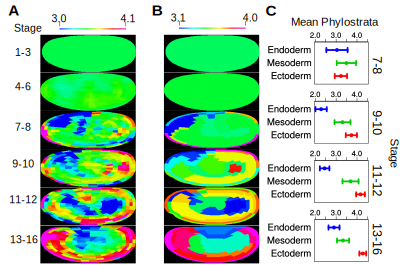
\includegraphics[width=0.7\textwidth]{./Images/Art-III/TAI.png}
  \centering
  \caption{\textbf{The center of the embryo expresses older genes.}
   (A) Heatmaps showing the transcriptome age index (TAI) im polar regions (B) Heatmaps showing the TAI for STs. (C) Mean phylostrata of genes assigned to each germ layer. Circles represent the mean and whiskers the SEM.
  }
  \label{fig:Art-III-TAI}
\end{figure}
	\nomenclature{SEM}{Standard error of the mean}
%%%%%%%%%%%%%%%%%%%%%%%%%%%%%%%%%%%%%%%%%%%%%%%%%%%%%%%%
%
%results TAI
I found that STs with low $\omega_{\alpha}$ express (on average) older genes (high TAI values; see Fig. \ref{fig:Art-III-TAI}). Similar results were found for anatomical structures (III, Fig. S2).
%
I also found that in stage 13-16 the mean phylogenetic age of the genes expressed in the endoderm is lower than in other germ-layers, specially compared to the ectoderm (Fig. \ref{fig:Art-III-TAI}).
Similar TAI results between germ-layers were found by \citet{Domazet-Loso2007} but without stages comparisons.
% discussion TAI
The correlation between adaptation and gene age fit the expectation that older genes would more likely perform essential functions than younger genes, and that, as older genes would have been moulded by natural selection for longer times would be therefore more close to optimality (assuming that this function is conserved). Therefore, more room for changes would be expectable in embryo regions with a larger proportion of younger genes. 

% results Codon Bias
I also found that embryo polar regions with high $\omega_{\alpha}$ have low codon bias (previously reported by  \citealp{Sharp1991,Betancourt2002,Haerty2007}) and that, as \citet{Plotkin2011} previously found, regions high codon bias show have high levels of gene expression (average RNAseq levels per region; III, methods).
To clarify the relation between these three variables, I fitted a multivariate linear regression and found that embryo regions with high $\omega_{\alpha}$ exhibit low codon bias relative to what would be expected from their gene expression levels (III, Fig 5).
%discussion codon bias
The negative correlation between codon bias and protein adaptation that I found would be expected given that, an adaptive  aminoacid change in a protein would be probably different from a change that would increase codon usage efficiency \citep{Hershberg2008,Presnyak2015}.
%Since codon bias also correlates with gene expression levels per region, high $\omega_{\alpha}$ should be found where codon usage is low relative to gene expression levels, as we observe

\subsection{Selective constraint in late embryogenesis} \label{OmegaA_late_embryo}

Analysing the RNAseq developmental data from the modENCODE project \citep{Graveley2011} with the DFE-alpha method (IV, methods), I found that from hour 10 until 24 of embryogenesis show significant low $\omega_{\alpha}$ and $\omega$ (see Fig X in section X), which would be consistent with the low rate of adaptive change seen in many anatomical structures in stage 13-16 (as stage 13-16 of BDGP roughly maps to RNA-seq samples em10-12 hr, em12-14 hr, em14-16 hr, and em16-18 hr of modENCODE; \citealp{Hammonds2013}).
Therefore, by combining different approaches, I could identify that the proteins produced in late embryogenesis change less their aminoacid sequence (i.e., are more conserved). This phenomenon, of some proteins evolving slower, has been called `selective constraint' and has been linked to the higher degree of functionality of such proteins \citep{kimura1983neutral}.
Most importantly, I could identify which specific anatomical structures expressed genes with a higher degree of conservation.